\documentclass[12pt, a4paper]{report}
\usepackage{caption, subcaption}
\usepackage[utf8]{inputenc}
\usepackage[italian]{babel}
\usepackage[T1]{fontenc}
\usepackage{graphicx}
\usepackage[top=3cm, bottom=3cm]{geometry}
\usepackage{tabularx}
\usepackage{titlesec}
\usepackage{colortbl}
\usepackage{csquotes}
\usepackage{amsmath}
\usepackage{amssymb}
\usepackage{xcolor}
\usepackage{array}
\usepackage{float}

\newcommand{\apj}{\textit{The Astrophysical Journal}}
\newcommand{\mnras}{\textit{Monthly Notices of the Royal Astronomical Society}}
\newcommand{\aap}{\textit{Astronomy \& Astrophysics}}
\newcommand{\nar}{\textit{New Astronomy Reviews}}
\newcommand{\araa}{\textit{Annual Review of Astronomy and Astrophysics}}

\usepackage[backend=biber, style=authoryear]{biblatex}
\addbibresource{bibliografia.bib}

\newcolumntype{C}[1]{>{\centering\arraybackslash}p{#1}}

\renewcommand*{\nameyeardelim}{\addspace}
\renewcommand*{\postnotedelim}{\addcolon\space}
\renewcommand*{\finentrypunct}{)}
\renewcommand{\chaptername}{Capitolo}

\begin{document}

L'obiettivo di questo lavoro di tesi è valutare le dimensioni e le eccentricità dei dischi proto-planetari circumstellari in dipendenza dei parametri del sistema binario che li ospita.
L'analisi da noi effettuata si concentra sul mass-ratio $q$, sull'eccentricità della binaria $e$ e sulla viscosità del materiale costituente il disco.

I dischi proto-planetari sono delle strutture sottili costituite da gas e polveri che orbitano attorno ad una stella e in essi si formano i pianeti.
L'evoluzione del disco è dettata da meccanismi che determinano una ridistribuzione del momento angolare: il materiale che lo costituisce accresce lentamente sul corpo centrale.
Se un sistema stellare è composto da due stelle gravitazionalmente legate, detto binario, si possono presentare tre dischi proto-planetari distinti: due circumstellari ed uno circum-binario.
Nell'ambito di questa tesi siamo interessati ai dischi circum-stellari, che abbiamo considerato come coplanari con le due stelle.

Determinare l'estensione spaziale di un disco d'accrescimento in un sistema multiplo è una problematica che può essere affrontata con diversi approcci.
L'interazione fra un corpo perturbante ed un disco di materiale gassoso è stata studiata con approcci semi-analitici considerando le forze di marea \parencite{PapaloizouPringle1977}, in termini di risonanze fra le orbite del disco e della binaria assumendo che le perturbazioni fossero eccitate in specifiche regioni spaziali del disco \parencite{GoldreichTremaine1980} oppure considerando tutta la fisica del problema mediante simulazioni numeriche \parencite{ArtymowiczLubow1994}.
Tali lavori hanno consentito di determinare che la posizione in cui avviene il troncamento dipende dall'eccentricità $e$ dell'orbita del sistema binario, dal mass-ratio $q$, dal parametro adimensionale $\alpha$ che regola la viscosità del materiale e dalla temperatura $T$ del disco. 
\cite{ManaraTronc2019} hanno proposto una formula analitica per la determinazione del raggio di troncamento
\begin{equation}
r_t\,=\,R_{L} (a e^b\,+\,c\mu^d),
\label{eq:tronc_disc}
\end{equation}
dove $R_L$ è la dimensione spaziale del Roche-Lobe \parencite{Eggleton1983}, $c\,=\,0.88$ e $d\,=\,0.01$ sono dei parametri determinati a partire dal lavoro di \cite{PapaloizouPringle1977} ed $a$, $b$ sono stati calcolati fittando i risultati numerici ottenuti da \cite{ArtymowiczLubow1994}.

Il sostegno computazionale allo studio del troncamento è esiguo. 
Le simulazioni effettuate in \cite{ArtymowiczLubow1994} per dischi circumstellari sono solamente otto caratterizzate da: $\mu\,\in\,\{0.1,\,0.3\}$, $e\,\in\,\{0.0,\,0.3\}$.
Un campionamento più fine dello spazio dei parametri è stato effettuato da \cite{Pichardo2005}: il metodo delle \textit{test particles} da loro utilizzato focalizza l'attenzione del loro lavoro su effetti puramente dinamici e non consente di studiare i fenomeni di natura viscosa che regolano l'evoluzione del disco.

Uno degli obiettivi di questa tesi è di ampliare il bagaglio simulativo a sostegno dello studio del troncamento.
I sistemi binari che abbiamo analizzato possono essere divisi in tre categorie: circolari ($e\,=\,0.0$), a media eccentricità ($e\,=\,0.3$) e ad elevata eccentricità ($e\,=\,0.6$).
Per ogni valore di $e$, abbiamo studiato quattro rapporti fra la massa $m_2$ della stella secondaria e quella $m_1$ della primaria: $m_2/m_1\,=\,0.1,\,0.33,\,0.5,\,1$.
A viscosità fissata i dischi presi in considerazione sono 21, in quanto nel caso di masse uguali per la primaria e la secondaria le caratteristiche dei due dischi sono le stesse.
Il numero totale di simulazioni effettuate in questo lavoro di tesi è 63, poiché abbiamo deciso di lavorare con tre differenti viscosità del materiale orbitante: abbiamo esplorato l'intervallo caratteristico del problema in analisi ponendo $\alpha\,\in\,\{10^{-2},\, 10^{-3},\,10^{-4}\}$.
L'evoluzione dei dischi è stata studiata per mezzo di FARGO3D \parencite{Fargo3D}, che è un codice a griglia euleriana sviluppato con l'obiettivo di studiare la fisica dei dischi d'accrescimento.
Le dimensioni del disco e la sua eccentricità vengono valutate per ogni configurazione assunta dal materiale fra il trentesimo e il cinquantesimo periodo di rivoluzione della binaria: i risultati che forniamo sono i valori medi delle stime effettuate.
Abbiamo determinato l'estensione dei dischi con due metodi differenti: per ogni sistema in analisi effettuiamo una stima del raggio di troncamento e del semiasse maggiore del disco. In Figura \ref{fig:sax_magg} sono riportati i valori di semiasse maggiore ottenuti per le tre viscosità considerate.

\begin{figure}[h]
    \centering
    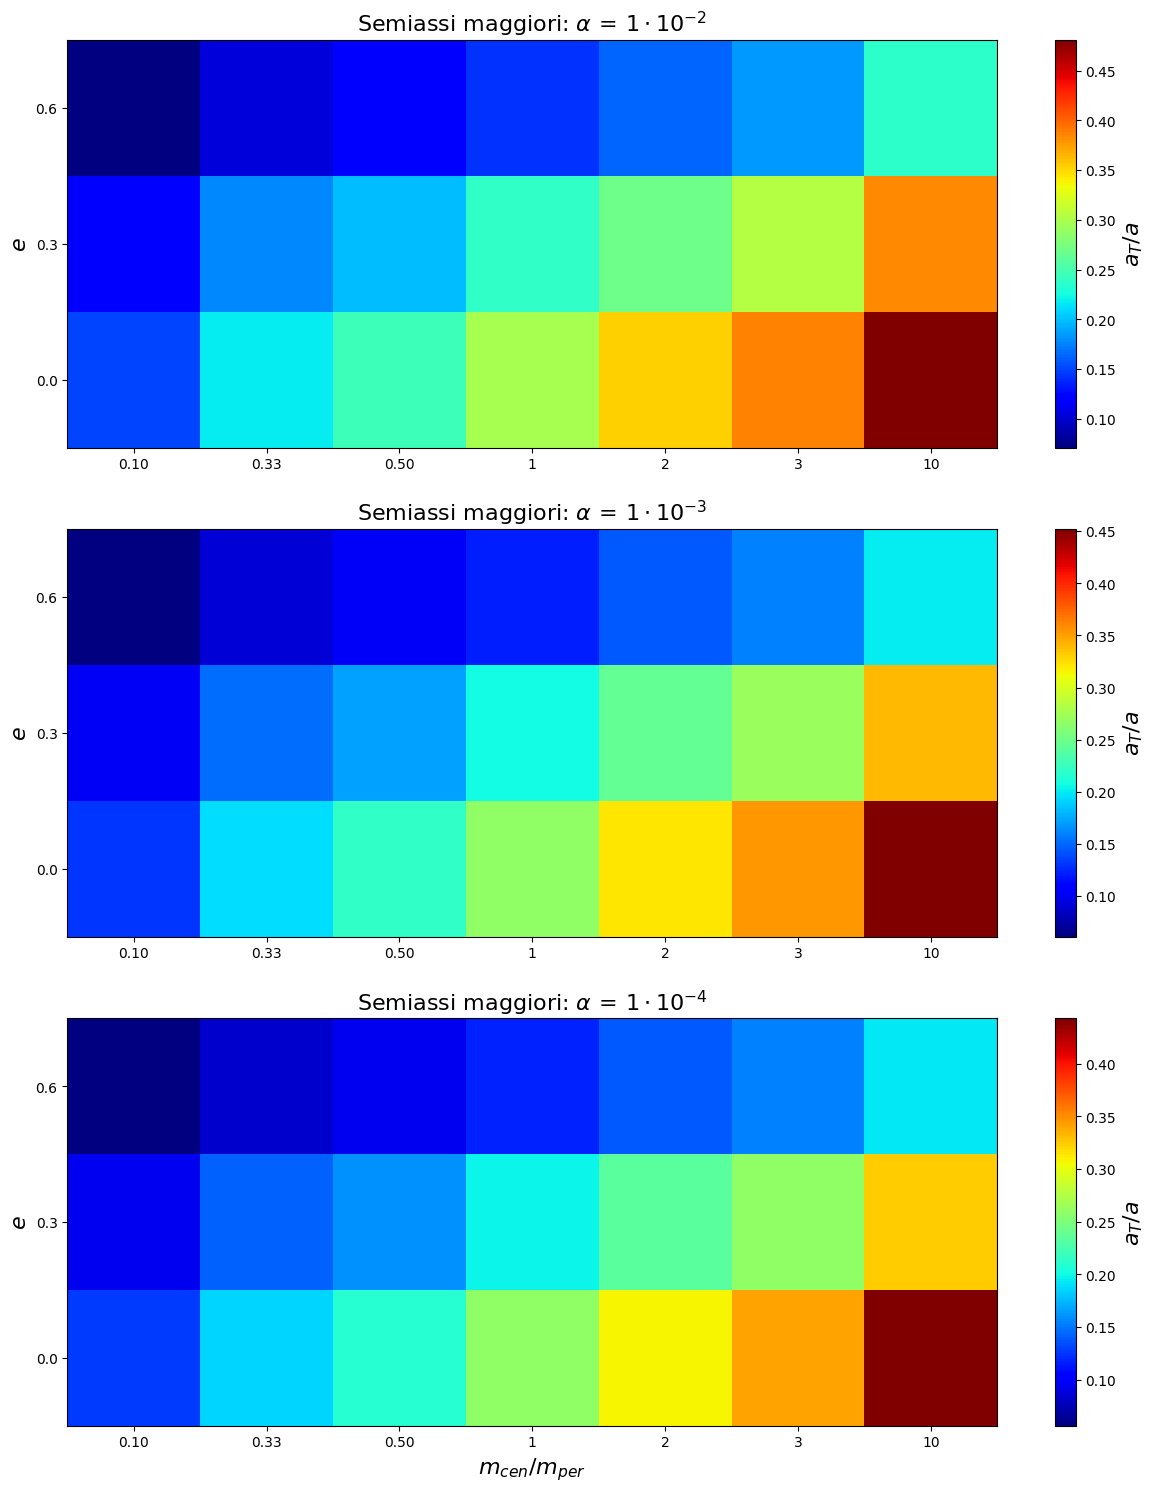
\includegraphics[width=\textwidth]{Immagini/graf_riass.png}
    \caption{In figura sono riportati i risultati ottenuti per i semiassi maggiori dei dischi: ogni grafico è dedicato ad un valore differente di $\alpha$. Sulle ascisse è posto il rapporto $m_{cen}/m_{per}$, dove $m_{cen}$ è la massa posta al centro della griglia, mentre $m_{per}$ quella del corpo perturbante. Notiamo come ad eccentricità della binaria fissata i dischi sono più grandi maggiore è la frazione di massa del sistema binario attorno alla quale orbitano. A $m_{cen}/m_{per}$ fissato, si può osservare una netta diminuzione delle dimensioni del disco all'aumentare di $e$.}
    \label{fig:sax_magg}
\end{figure}

Osserviamo che ad $e$ fissato, la dimensione del disco dipende fortemente dal valore di $m_{cen}/m_{per}$, dove $m_{cen}$ è la massa della stella al centro della griglia, mentre $m_{per}$ la massa del corpo perturbante: i dischi che orbitano attorno ad una frazione di massa della binaria più elevata sono più grandi.
All'aumentare di $e$ le dimensioni dei dischi circumstellari analizzati diminuiscono sensibilmente: questo andamento è dovuto al fatto che le risonanze eccentriche sono di intensità maggiore per un sistema ad alta $e$, con un conseguente spostamento della regione di troncamento \parencite{ArtymowiczLubow1994}.
\'E possibile osservare una dipendenza da $\alpha$: maggiore è la viscosità, maggiori sono le dimensioni del disco che otteniamo.

La seconda caratteristica a cui siamo interessati è $e_{disco}$: abbiamo definito come $e_{disco}$ l'eccentricità delle orbite percorse dal materiale nell'intorno del semiasse maggiore del disco.
Abbiamo effettuato una stima per ognuno dei 63 dischi simulati, osservando che in media $e_{disco}$ diminuisce all'aumentare dell'eccentricità della binaria: questo accade perché i dischi sono soggetti ad un troncamento maggiore e le risonanze che eccitano l'eccentricità dell'oggetto orbitante possono non trovarsi più nella regione da esso occupato.

Abbiamo effettuato un confronto fra le dimensioni dei dischi da noi ottenute e quelle presenti in letteratura osservando un buon accordo per quelli ospitati in sistemi binari a media o elevata eccentricità. 
Nel caso di binaria circolare la teoria descrive correttamente il modo di scalare delle dimensioni del disco in dipendenza di $m_2/m_1$, ma sono presenti discrepanze del $10/15\,\%$ fra valori i valori presenti in letteratura e quelli simulati.
Considerato il buon accordo fra i nuovi risultati numerici e quelli ottenuti da lavori precedenti, uno dei possibili sviluppi futuri di questa tesi è un estensione del fit di $a,\,b\,c,\,d$ ad una nuova regione dello spazio dei parametri.

\end{document}
